\chapter{Fundamentos del lenguaje}


\section{Python}

Python es un lenguaje de programación, interpretado, de alto nivel y propósito general, además de ser un proyecto  
libre y de código abierto, con una comunidad enorme implicada en el desarrollo y mantenimiento de librerías que hacen 
posible el \textit{multidominio} actual de Python.

Dada su concepción como lenguaje de propósito general, Python es utilizado en una diversidad de aplicaciones, 
desde desarrollo web, encriptación, análisis de datos, procesamiento de imágenes, aprendizaje automático, 
computación simbólica, etc.  

Las características de este lenguaje le hacen propicio para el prototipado de aplicaciones, dado que es muy 
sencillo y rápido revisar y modificar el código desarrollado. Otra característica muy notable de Python 
es su sintaxis simple y fácil de aprender, lo cual ayuda al momento de introducirse en el desarrollo de 
algoritmos o el mundo propio de la programación de computadoras.

\section{Instalando Python}

En estos apuntes se utilizará la distribución Anaconda de Python, la cual contiene el intérprete y las librerías del 
\textit{core}, pero además incluye la mayoría de librerías utilizadas para el desarrollo de aplicaciones de corte 
técnico-científico.

La descarga de Anaconda puede realizarla desde el sitio \url{https://www.anaconda.com/download/}, selecciona el 
paquete de descarga conforme al sistema operativo (Windows, macOS o Linux) así como la arquitectura de su PC.
La instalación suele ser muy sencilla, puede seguir las instrucciones dadas en el \textit{How to install ANACONDA} de 
la misma página.

\section{La consola de Python como una calculadora básica}

Una vez instalado Anaconda puede testear la correcta instalación abriendo \textbf{Anaconda Prompt}, la cual es 
una consola desde la cual puede ejecutar algunos Scripts que complementan el funcionamiento de Python. Puede 
buscar esta consola en la carpeta de instalación correspondiente. Cuando la ejecute observará una consola 
como la mostrada en la figura \ref{fig:anaconda_prompt}

\begin{figure}[h!]
	\centering
	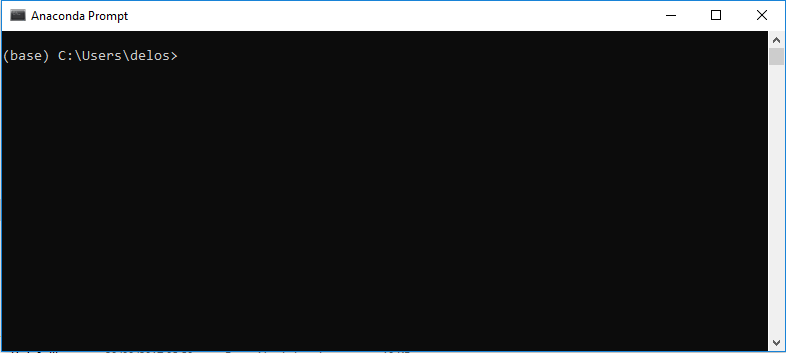
\includegraphics[width=0.75\textwidth]{img/ch01/anaconda_prompt.png}
	\caption{Anaconda Prompt}
	\label{fig:anaconda_prompt}
\end{figure}

Dentro de esta consola escriba \texttt{python} y presione la tecla \textbf{Enter}, al hacer esto observará 
que la consola cambia el prompt compuesto de un directorio por tres signos de \textit{mayor que} tal como 
se puede verificar en la figura \ref{fig:anaconda_prompt_python}.

\begin{figure}[h!]
	\centering
	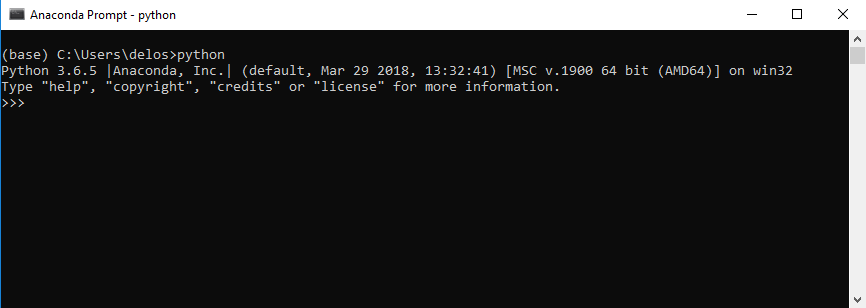
\includegraphics[width=0.75\textwidth]{img/ch01/anaconda_prompt_python.png}
	\caption{Consola Python}
	\label{fig:anaconda_prompt_python}
\end{figure}

A partir de este momento puede ingresar código Python y teclear \textbf{Enter} para ejecutar la instrucción  
y la consola le devolverá lo que resulte de esto. Por ejemplo, si escribe un número cualesquiera y presiona enter, 
la consola le devolverá justamente el mismo número:

\begin{python}
>>> 1000
1000
\end{python}

Puede ejecutar un simple suma aritmética:

\begin{python}
>>> 100 + 200
300
\end{python}

O una resta:

\begin{python}
>>> 550 - 650
-100
\end{python}

Naturalmente Python maneja sin complicaciones las cantidades negativas. Una multiplicación la realiza 
con el operador *:

\begin{python}
>>> 50*25
1250
\end{python}

Para las divisiones utiliza el operador /:

\begin{python}
>>> 1/2
0.5
\end{python}

Puede elevar a una potencia utilizando como operador el doble asterisco:

\begin{python}
>>> 13**2
169
\end{python}

Inclusive existe la posilidad de definir números complejos y realizar operaciones con ellos:

\begin{python}
>>> 5 + 2j
(5+2j)
>>> (5 + 2j) - (10 + 7j)
(-5-5j)
>>> (5 + 2j)*(10 + 7j)
(36+55j)
\end{python}

Puede ampliar la capacidad de las funcionalidades \textit{built-in} de Python si importa alguna librería, como 
\texttt{math}, pero claro, eso será un tema a tratar con posterioridad.

\section{Variables y tipos de datos}

Al ser un lenguaje de alto nivel, Python dispone de los tipos de datos elementales en cualquier lenguaje de programación, 
pero además incluye estructuras de datos muy \textit{avanzadas} y con altas prestaciones que facilitan en muchos 
aspectos la tarea del programador.

Python es un lenguaje de tipado dinámico en el que no hace falta declarar el tipo de dato que asignará a una variable, 
de igual manera una variable puede cambiar de tipo conforme la ejecución del programa, por ello se debe tener cuidado 
con la sintaxis para definir cada tipo de dato.

\subsection{Variables}

Las variables son referencias a los objetos de Python, son creadas por asignación mediante el signo \texttt{=}, 
por ejemplo:

\begin{python}
>>> a = 2
>>> b = 10
>>> a + b
12
\end{python}

El nombre de una variable puede constar de una combinación de caracteres alfanúmericos y el guión bajo, 
siempre y cuando el primer caracter no sea un dígito. Además, en Python los nombres de variables son 
\textit{case sensitive}, es decir, se distingue entre mayúsculas y minúsculas.

\begin{python}
>>> D = 177.8
>>> d = 95
>>> print(D)
177.8
>>> print(d)
95
\end{python}

Existen algunas palabras reservadas del lenguaje que no puede utilizar como nombre de variable, 
puede verificar cuáles son estas palabras tecleando lo siguiente:

\begin{python}
>>> import keyword
>>> keyword.kwlist
['False', 'None', 'True', 'and', 'as', 'assert', 'break', 'class', 'continue', 'def', 'del', 'elif', 'else', 'except', 'finally', 'for', 'from', 'global', 'if', 'import', 'in', 'is', 'lambda', 'nonlocal', 'not', 'or', 'pass', 'raise', 'return', 'try', 'while', 'with', 'yield']
\end{python}


\subsection{Enteros}



\subsection{De coma flotante}



\subsection{Cadenas de caracteres}

Las cadenas de caracteres (denominadas habitualmente y de manera indistinta como \textit{strings}) es un tipo de dato 
que contiene una secuencia de símbolos, mismos que pueden ser alfanúmericos hasta cualquier otro símbolo propio de 
un sistema de escritura. En Python los strings se definen entre comillas dobles o simples:

\begin{python}
>>> "esta es una cadena de caracteres"
'esta es una cadena de caracteres'
>>> 'esta también'
'esta también'
\end{python}

Puede concatenar dos strings utilizando el operador \texttt{+}:

\begin{python}
>>> "Hola" + "mundo"
'Holamundo'
\end{python}

Notará que Python por sí mismo no sabe que estamos uniendo dos palabras y que entre ellas debería haber un espacio 
para su correcta lectura, evidentemente este tipo de cuestiones son las que el programador debe tomar en cuenta al 
escribir un código.

Una cadena de caracteres es lo que en Python se conoce como \textit{iterable}, es decir, una secuencia de 
elementos agrupados a los cuales se puede acceder de manera individual mediante indexación. Por ejemplo, 
sea \texttt{nombre} una cadena de caracteres dada por:

\begin{python}
>>> nombre="Catalina"
\end{python}

Puede acceder a cada una de las letras que componen dicha cadena mediante la notación \texttt{iter[pos]}, donde 
\texttt{iter} es el nombre del iterable y \texttt{pos} la posición en que se encuentra el caracter al cual 
se desea acceder, siendo 0 para la primera letra, 1 para la segunda y así de manera consecutiva. Por ejemplo: 

\begin{python}
>>> nombre[0]
'C'
>>> nombre[4]
'l'
>>> nombre[2]
't'
\end{python}

Al último elemento, sin importar la longitud de la cadena, se accede con el índice -1:

\begin{python}
>>> nombre[-1]
'a'
\end{python}


\subsection{Booleanos}



\subsection{Listas}

Las listas son estructuras de datos que pueden almacenar cualquier otro tipo de dato, inclusive una lista 
puede contener otra lista, además, la cantidad de elementos de una lista se puede modificar removiendo o 
añadiendo elementos. Para definir una lista se utilizan los corchetes, dentro de estos se colocan todos 
los elementos separados por comas:

\begin{python}
>>> calificaciones = [10,9,8,7.5,9]
>>> nombres = ["Ana","Juan","Sofía","Pablo","Tania"]
>>> mezcla = [True, 10.5, "abc", [0,1,1]]
\end{python}

Las listas son iterables y por tanto se puede acceder a sus elementos mediante indexación:

\begin{python}
 >>> nombres[2]
'Sofía'
>>> nombres[-1]
'Tania'
\end{python}

Se tiene la posibilidad de agregar elementos a una lista mediante el método \code{append}: 

\begin{python}
>>> nombres.append("Antonio")
>>> nombres.append("Ximena")
>>> print(nombres)
['Ana', 'Juan', 'Sofía', 'Pablo', 'Tania', 'Antonio', 'Ximena']	
\end{python}

El método \code{remove} elimina un elemento de una lista:

\begin{python}
>>> nombres.remove("Ana")
>>> print(nombres)
['Juan', 'Sofía', 'Pablo', 'Tania', 'Antonio', 'Ximena'] 	
\end{python} 

Sí el valor pasado al método \code{remove} no existe, Python devolverá un \code{ValueError}:

\begin{python}
>>> nombres.remove("Jorge")
Traceback (most recent call last):
  File "<stdin>", line 1, in <module>
ValueError: list.remove(x): x not in list
\end{python}



\subsection{Tuplas}

Las tuplas son secuencias de elementos similares a las listas, la diferencia principal es que 
las tuplas no pueden ser modificadas directamente, es decir, una tupla no dispone de los métodos 
como \code{append} o \code{insert} que modifican los elementos de una lista.

Para definir una tupla, los elementos se separan con comas y se encierran entre paréntesis.

\begin{python}
>>> colores=("Azul","Verde","Rojo","Amarillo","Blanco","Negro","Gris")
\end{python}

Las tuplas al ser \textit{iterables} pueden accederse mediante la notación de corchetes e índice.

\begin{python}
>>> colores[0]
'Azul'
>>> colores[-1]
'Gris'
>>> colores[3]
'Amarillo'
\end{python}

Si intentamos modificar alguno de los elementos de la tupla Python nos devolverá un \code{TypeError}:

\begin{python}
>>> colores[0] = "Café"
Traceback (most recent call last):
  File "<stdin>", line 1, in <module>
TypeError: 'tuple' object does not support item assignment
\end{python}


\subsection{Diccionarios}

Los diccionarios son estructuras que contienen una colección de elementos de la 
forma \textit{clave: valor} separados por comas y encerrados entre llaves. 
Las claves deben ser objetos inmutables y los valores pueden ser de cualquier tipo. 
Necesariamente las claves deben ser únicas en cada diccionario, no así 
los valores. 

Vamos a definir un diccionario llamado \code{edades} en el cual 
cada clave será un nombre y el valor una edad:

\begin{python}
>>> edades = {"Ana": 25, "David": 18, "Lucas": 35, "Ximena": 30, "Ale": 20}
\end{python}

Puede acceder a cada valor de un diccionario mediante su clave, por ejemplo, 
si quisieramos obtener la edad de la clave \code{"Lucas"} se tendría que escribir:

\begin{python}
>>> edades["Lucas"]
35
\end{python}


\section{Operadores relacionales y lógicos}


\section{Control de flujo}

\subsection{Condicional if-elif-else}

El condicional \code{if-elif-else} es una estructura de control que sirve para tomar decisiones 
en el flujo del programa. La sintaxis para \code{if-elif-else} es:

\begin{python}
if cond1:
    # hacer algo 
elif cond2:
    # hacer otra cosa
    .
    .
    .
elif condn:
    # hacer algo más
else:
    # hacer algo por default
\end{python}

Donde \code{cond1, cond2, ... condn} son valores lógicos que resultan de una comparación. Esta estructura se evalúa 
secuencialmente hasta encontrar una condición que se cumpla, si ninguna lo hace, entonces se ejecuta la instrucción 
colocada en el caso por default \code{else}.



\subsection{Bucle for}

El \textbf{bucle for} es una estructura de control de naturaleza repetitiva, en la cual se conocen 
\textit{a priori} el número de iteraciones a realizar \footnote{Aunque no sea tan habitual, un bucle for en Python puede 
romperse mediante instrucciones explícitas de interrupción de ejecución}. 

En lenguajes como C++ o Java, el ciclo for necesita de una variable de ciclo de tipo entero 
que irá incrementándose en cada iteración. En Python, la cuestión es un poco diferente, el ciclo 
for \textit{recorre} un \textit{iterable} y en la k-ésima iteración la variable de ciclo \textit{adopta} el 
valor del elemento en la k-ésima posición del iterable.

De manera general, la sintaxis de for es:

\begin{python}
for var in iterable:
    # Hacer algo ...
\end{python}

Donde \code{var} es la \textbf{variable de ciclo} e \code{iterable} la secuencia de valores que deberá iterarse. 
Es necesario remarcar la importancia de los dos puntos al final de esta primera línea y en indentar el bloque de 
código subsecuente que definirá el cuerpo del ciclo for.

Como primer ejemplo vamos a recorrer una lista de números y mostrarlos por consola:

\begin{python}
numeros = [18,50,90,-20,100,80,37]
for n in numeros:
    print(n)
\end{python}
\begin{outscript}
18
50
90
-20
100
80
37
\end{outscript}

Observe que en cada iteración la variable de ciclo \code{n} adopta el valor de cada uno de los elementos de la 
lista \code{numeros}.

Como ya se mencionó, en Python la variable de ciclo no necesariamente adopta valores numéricos enteros secuenciales, 
si no valores dentro de una secuencia. Esta secuencia podría ser también una cadena de caracteres, por ejemplo:

\begin{python}
palabra = "Python"
for letra in palabra:
    print(letra)
\end{python}
\begin{outscript}
P
y
t
h
o
n
\end{outscript}

Dentro de un ciclo for podemos colocar cualesquiera otra instrucción de control de flujo. Un caso 
muy común es el de incluir otro ciclo for, algo que habitualmente se denota como \textbf{ciclos anidados}. 
Por ejemplo, supongamos que se requieren mostrar por consola todos los elementos de algunas listas contenidas 
dentro de otra lista principal, en ese caso se hace necesario primero iterar sobre la lista principal y 
enseguida hacerlo sobre las listas contenidas, por ejemplo:

\begin{python}
matriz = [[-5,2,0], [9,5,6], [1,7,15]]
for fila in matriz:
    for elemento in fila:
        print(elemento)
\end{python}
\begin{outscript}
-5
2
0
9
5
6
1
7
15
\end{outscript}




\subsection{Bucle while}



\section{Funciones}

Las funciones son \textit{porciones de código} nos sirven para modularizar 
nuestros programas y evitar en muchos casos la repetitividad de código. 
De manera general una función recibe algunos valores de entrada, los \textit{procesa} y 
devuelve algunos valores de salida. 

\subsection{Funciones nativas de Python (\textit{built-in})}

Python dispone de algunas funciones nativas que se \textit{cargan} automáticamente cuando se 
inicia el intérprete. Por ejemplo la función \code{max} devuelve el mayor valor numérico de 
una lista de números:

\begin{python}
>>> max([10,35,5,110,48,30,112,98,87])
112
\end{python}

También existe una función \code{min}, análoga a \code{max}:

\begin{python}
>>> min([10,35,5,110,48,30,112,98,87])
5
\end{python}

Otro ejemplo de función nativa es \code{bin}, la cual dado un número en base 10 devuelve 
una cadena con la representación en base 2.

\begin{python}
>>> bin(10)
'0b1010'
\end{python}

Naturalmente, el valor devuelto por una función se puede asignar a una variable y posteriormente ser utilizado:

\begin{python}
>>> a = max([10,5,8])
>>> b = min([10,5,8])
>>> h = (a - b)/10
>>> print(h)
0.5
\end{python}

Hay funciones como \code{print} que no devuelven como tal un valor, si no que pueden modificar directamente 
alguna variable global o simplemente mostrar algo en la salida estándar como el caso de \code{print}.

Tendremos también funciones que aceptan más de un argumento, por ejemplo a la función \code{round} podemos 
pasarle dos argumentos: un número real y la cantidad de lugares decimales a considerar para el redondeo.

\begin{python}
>>> round(3.141592653589793, 6)
3.141593
>>> round(3.141592653589793, 4)
3.1416
>>> round(3.141592653589793, 2)
3.14
>>> round(3.141592653589793, 0)
3.0
\end{python}



\subsection{Funciones definidas por el usuario}

Además de las funciones nativas de Python, es posible definir nuestras propias funciones. 
En Python, de manera general, una función se define siguiendo la estructura mostrada a continuación:

\begin{python}
def nombre_fun(arg1, arg2, ..., argN):
	# Cuerpo de la función
	# .
	# .
	# .
	return val1, val2, ..., valN
\end{python}

Donde \code{def} es una palabra que debe anteceder siempre a la definición de una función, 
\code{nombre\_fun} es el nombre que se asignará a la función, entre paréntesis y 
separados por comas se colocan los nombres de los argumentos de entrada, los dos puntos 
se colocan después de cerrar el paréntesis e indican que ahí termina el \textit{encabezado} de 
la función y comenzará el \textit{cuerpo} de la misma, aquí se colocarán todas las 
instrucciones que deberán realizarse; la palabra reservada \code{return} sirve para 
indicar los valores a devolver, mismos que se colocarán separados por comas.

Vamos a definir una función llamada \code{saluda}, la cual recibe un nombre (string)
y devuelve un saludo (string) formado mediante concatenación:

\begin{python}
def saluda(nombre):
    s = "Hola " + nombre + ", bienvenido."
    return s

print(saluda("Jorge"))
\end{python}
\begin{outscript}
Hola Jorge, bienvenido.
\end{outscript}

Lo único que hace la función anterior es tomar un \textit{string} como argumento y unirlo 
a algunas cadenas ya establecidas dentro de la función. 

Veamos ahora cómo definir una función que recibe como argumento un entero y devuelve un valor lógico que 
indica si este es par.

\begin{python}
def espar(n):
    if n%2 == 0:
        s = True
    else:
        s = False
    return s

print(espar(2))
print(espar(5))
print(espar(10))
\end{python}
\begin{outscript}
True
False
True
\end{outscript}


Naturalmente, las funciones pueden recibir más de un argumento. Por ejemplo:

\begin{python}
def mayor(a,b):
    m = a
    if a < b:
        m = b
    return m

print( mayor(50,30) )
print( mayor(1100,3050) )
\end{python}
\begin{outscript}
50
3050
\end{outscript}

La función \code{mayor} recibe dos valores numéricos y determina cuál es el mayor de ambos mediante 
una comparación con la sentencia \code{if}. 

¿Pueden las funciones en Python devolver más de un valor? ¡Claro! Hace falta nada más separar 
con comas los valores a devolver.

\begin{python}
def calcula_rectangulo(b,h):
    A = b*h
    P = 2*b + 2*h
    return A, P

print( calcula_rectangulo(10,5) )
print( calcula_rectangulo(50,15) )
\end{python}
\begin{outscript}
(50, 30)
(750, 130)
\end{outscript}

También es posible guardar/asignar los valores devueltos por la función en variables:

\begin{python}
area1, perimetro1 = calcula_rectangulo(100, 20)
print("Área: {0}\nPerímetro: {1}".format(area1, perimetro1))
\end{python}
\begin{outscript}
Área: 2000
Perímetro: 240
\end{outscript}


\subsubsection{Funciones con una cantidad de parámetros indeterminada}

En ocasiones el número de parámetros que deberá recibir una función no puede ser algo fijo. 
Las definiciones de función en Python tienen la flexibilidad de poder recibir una cantidad 
variable de argumentos de entrada. 

Para ejemplificar esto, vamos a crear una función llamada \code{promedio} que calcule 
el promedio de una cierta cantidad de números pasados como argumentos:

\begin{python}
def promedio(*numeros):
    suma = 0
    k = 0
    for n in numeros:
        suma += n
        k += 1
    return suma/k

print(promedio(10,5))
print(promedio(10,50,40,80,20,100))
print(promedio(5,15,10,5))
\end{python}
\begin{outscript}
7.5
50.0
8.75
\end{outscript}

Observe que lo único que hacemos es que al nombre del parámetro le anteponemos un asterisco, esto le indica 
a Python que la cantidad de argumentos de entrada es indeterminada, en principio. Claro está, que el manejo posterior 
de la información es algo que el programador debe tener en cuenta. Dentro del cuerpo de la función 
se debe considerar que el parámetro \code{numeros} será una tupla cuya cantidad de elementos dependerá 
de la cantidad de argumentos ingresados.


\subsubsection{Funciones y los argumentos con nombre}

Una función en Python se puede \textit{mandar a llamar} pasándo los argumentos de manera posicional, es 
decir, en el orden que fueron definidos en la función, o bien, haciendo uso del nombre del parámetro correspondiente 
al argumento que se introduce, por ejemplo:

\begin{python}
def cuenta_cuantas(frase, letra):
    k = 0
    for car in frase:
        if car is letra:
            k += 1
    return k

print( cuenta_cuantas("hola mundo", "o") )
print( cuenta_cuantas(frase="hola mundo", letra="o") )
print( cuenta_cuantas(letra="o", frase="hola mundo") )
\end{python}

La función \code{cuenta\_cuantas} devuelve el número de presencias de una determinada letra en una frase. Observe 
las tres formas en que la \textit{ejecutamos}, todas son equivalentes. En la primera se pasan los argumentos de 
forma posicional, en la segunda y tercera se utilizan los argumentos con nombres, note que en este caso el orden 
en que los argumentos son pasados, es indistinto.

En la definición de funciones es posible también especificar que se pasarán ciertos argumentos con nombre 
sin necesidad de escribirlos de manera explícita. Observe la siguiente función:

\begin{python}
def muestra_puntos(**personas):
    for persona in personas.items():
        print(persona[0] + " tiene " + str(persona[1]) + " puntos")

muestra_puntos(Jorge=8, Paty=10)
print(30*"=")
muestra_puntos(Ana=6, Carlos=9, Victor=4, Daniela=8)
\end{python}
\begin{outscript}
Jorge tiene 8 puntos
Paty tiene 10 puntos
==============================
Ana tiene 6 puntos
Carlos tiene 9 puntos
Victor tiene 4 puntos
Daniela tiene 8 puntos
\end{outscript}

Vea que la definición de la función \code{muestra\_puntos} incluye un parámetro llamado \code{**personas}, esos dos 
asteriscos antes del nombre del parámetro, indican que no se tiene predeterminado el número de argumentos que se 
pasarán, pero además, indica que cada argumento a introducir deberá ser un argumento con nombre.
Dentro del cuerpo de la función el parámetro \code{**personas} es un diccionario cuyas claves 
son los nombres de los argumentos y los valores corresponden a cada valor asignado al argumento.



\section{Ejercicios}


\begin{enumerate}

% \textbf{Estructuras de control}

\item En las siguientes opciones se muestran operaciones aritméticas entre diversos 
objetos de Python. Verifique si es posible realizarlas e indique el resultado, 
de no ser así describa el por qué.

\begin{enumerate}
    \item \code{1 + 2}
    \item \code{1.3 + 2.5}
    \item \verb|"1" + 2|
    \item \verb|"1" + "2"|
    \item \code{[1,2,3] + [10,20]}
    \item \verb|{"a":10, "b":5} + {"h":2, "i":4}|
\end{enumerate}

\item Observe el siguiente código:

\begin{python}
for a,b in [1,2,5,3,8,7]:
    print(a)
\end{python}

Identifique y explique el error.

\item El siguiente código debería imprimir la longitud de cada palabra contenida en la 
lista \code{palabras}. Identifique el error.

\begin{python}
palabras = ["Carro", "Sol", "Mesa", "Dinosaurio", "Girasol", "Silla"]
for palabra in palabras:
    print(len(palabras))
\end{python}

\item Implemente un programa que determine si un número dado es par o impar.

\item Escriba un programa que cuente el número de vocales en una frase. Tome en cuenta que las vocales 
podrían ser tanto mayúsculas como minúsculas.

\item Escriba un programa que aproxime, mediante la suma de Riemann, el área bajo la curva de la función 
$ f(x) = x^2 + 3x $ en el intervalo $ 0 \leq x \leq 10 $. 

\end{enumerate}